\section{Statistical Generation as Planning}
\label{sec:pcrisp}

We now extend {\sc crisp} to statistical generation ({\sc pcrisp}). The basic idea is to add a statistical grammar model while leaving the sentence generation mechanism untouched. This way we can select the highest scoring derivation, that satisfies all constraints (grammaticality, expresses the communicative goal, use unambiguous referring expressions etc.). 

 As a straightforward probability model over {\sc ltag} derivations we choose probabilistic {\sc tag} ({\sc ptag}) \cite{resnik1992}.
Our choice of {\sc ptag} for sentence generation is motivated by a number of attractive properties.
 {\sc Ptag} is lexicalized and therefore does not only assign probabilities to operations in the grammar (as for example plain {\sc pcfg}), but also accounts for binary dependencies between words.  Unlike n-gram models however, these co-occurrences are structured according to local syntactic context as a result of {\sc tag}'s extended domain of locality. The probability model describes how the syntactic arguments of a word are typically filled. 
Furthermore, as {\sc tag} factors recursion from the domain of dependencies, the probability for core constructions remains the same independent of additional adjunctions. 
%Second, {\sc ptag} is a generative model. This is crucial because it allows us to assign probabilities to partial derivations. In addition we use the probability of partial derivations as a cost function, to help guide search through the space of possible PLTAG derivations. In contrast, other statistical generation systems use discriminative models that select the best possible generation output from a set of candidate sentences.
%Finally, the independence assumption makes it easy to estimate {\sc ptag}s from a treebank.
 We review {\sc ptag} in section \ref{ssec:probmodels}.

While we leave the basic sentence generation mechanism intact, we need to modify the concrete formulation of {\sc crisp} planning operators, as each of them now corresponds to some probability event. Likewise, we need to take the step from classical planning to metric planning systems, that can use the probabilities.
In metric planning \cite{fox2002}, instead of changing only boolean state variables, planning actions can decrease or increase a numeric variable. The goal state specifies constraints on this variable. In the simplest case the variable can only be increased by a static cost value in each action, and the goal state contains the objective to minimize the total cost. Systems such as metric-{\sc FF} \cite{hoffmann2003} do not guarantee optimality, but generally offer good results. We address our encoding of sentence generation with {\sc ptag} as metric planning in section \ref{ssec:pcrisp-domains}. 

\subsection{Probabilistic TAG}
\label{ssec:probmodels}
{\sc ptag} \cite{resnik1992} views {\sc tag} derivations as sequences of probability events of three types, initial events, substitution events and adjunction events.

\newcommand{\adj}[0]{\textit{ adj}}
\newcommand{\init}[0]{\textit{ init}}
\newcommand{\subst}[0]{\textit{ subst}}
The probability distribution for initial events describes how likely it is to start any derivation with a given initial tree. 
It is defined over all initial trees $\alpha$ with their possible lexicalizations $w \in W_\alpha$: 
$$ \sum\limits_{\alpha \in I}\sum\limits_{w \in W_\alpha} P_{init}(\init(\alpha, w)) = 1 $$

For substitution events, there is a probability distribution for each substitution node $n$ of each initial tree $\tau$ lexicalized with $v$, which describes how likely it is to substitute it with an initial tree $\alpha$ lexicalized with $w$. 
$$\sum\limits_{\alpha \in I}\sum\limits_{w \in W_\alpha} P_{subst}(\subst(\tau,v , \alpha, w, n)) = 1$$

Similarly for each internal node there is a distribution that describes the probability to adjoin each auxiliary tree $\beta$ lexicalized with $w$. In addition some probability mass is reserved for the event of not adjoining anything to such a node at all.

$$ P_{adj}(\adj(\tau, v, \textit{None}, n)) +$$
$$ \sum\limits_{\beta \in A}\sum\limits_{w_\beta} P_{adj}(\adj(\tau, v, \beta, w, n)) = 1.$$

{\sc Ptag} assumes that all events occur independent of each other. Therefore it defines the total probability for a derivation as the product of the probability of its individual events. 

\subsection{PCRISP Planning Domains}
\label{ssec:pcrisp-domains}
Using the definition of {\sc ptag}, we now reformulate the {\sc crisp} planning operators described in section \ref{ssec:crispdomain}.
The independence assumption in {\sc ptag} allows us to maintain that planning operator add a single tree, but are now assigned a probability score. However, while {\sc crisp} planning operators can add an elementary tree to any site of the right category, {\sc ptag} substitution and adjunction events are binary events between lexicalized trees at a specific node. We therefore adapt the literals that record open substitution and adjunction sites in partial derivations accordingly and create one operator for each node in each possible combination of lexicalized trees.
Figure \ref{example-action} shows an example planning operator for each type.
\begin{figure}[t]
\begin{center}
\cplanaction{\bf subst-t3-cat-t28-eats-n1(u,~x1)}{referent(u,~x1),\\ subst(t28-eats,~n1,~u), cat(x1)}{
$\lnot$needtoexpr(pred-cat,~x1),\\ $\lnot$subst(t-28-eats, n1,~u),\\
adj(t3-cat, n2 u)}{4.3012}\\\smallskip

\cplanaction{\bf adj-t5-raw-t3-fish-n2(u,~x1)}{referent(u,~x1),\\ adj(t28-eats,n2,~u), raw(x1)}{
$\lnot$needtoexpr(pred-raw,~x1),\\ $\lnot$adj(t-28-eats, n2,~u)}{6.9076}\\\smallskip

\cplanaction{\bf init-t28-eats(u,~x1,~x2,~x3)}{referent(u,~x1),\\ eats(x1,~x2,~x3)}{
$\lnot$needtoexpr(pred-eats,~x1,~x2,~x3), \\
 subst(t-28-eats,~n1,subj), subst(t28-eats,~n4,obj),\\
adj(t-28-eats, n2, u), adj(t-28-eats, n3, u)}{8.5172}\\\smallskip

\cplanaction{\bf noadj-t28-eats-n3(u)}{
 adj(t-28-eats,~n3,u)}
{$\lnot$ adj(t-28-eats, n3, u)}{0.1054}\\\smallskip

\caption{\label{example-action} {\sc pcrisp} Operator to substitute $t3$ lexicalized with 'cat' for node 2 of $t28$ lexicalized with `eats'.}
\end{center}
\end{figure}

Finally, we set the cost of an operator to be its negative log probability. For example for the operator in figure \ref{example-action} $$Cost( \subst(t_3,\textit{`cat'},t_{28},\textit{`eats"},n_2) ) =$$
$$ -\log( P(\subst(t_3,\textit{`cat'},t_{28},\textit{`eats"},n_2)) ). $$ This way the plan with the smallest cost sum corresponds to the {\sc tag} derivation with the highest probability. 

\subsection{Dealing with Data Sparseness}
\label{ssec:sparseness}
%To alleviate data sparseness, caused by the specific event definition of {\sc ptag}, we propose two alternative probability models. The first model is an unlexicalized version of {\sc ptag}, the second model uses a simple smoothing approach.\\ 
The probability event definition of {\sc ptag} is very fine grained. Substitution and adjunction events depend on specific parent and child trees with specific lexicalizations and on a node in the parent tree, as illustrated in figure \ref{fig:modelillustration}, B.1. When we estimate a probability model from training data, we cannot expect to observe evidence for all combinations of trees. Derivations that include such unseen events, have zero probability and are therefore impossible. As we show in section \ref{sec:experiments}, this gives rise to a massive data sparseness problem.

  A straightforward way to deal with data sparseness is to drop all lexicalizations from event definitions, as illustrated in figure \ref{fig:modelillustration}, A. Unfortunately this model does no longer account for bilexical dependencies between words. Since our system has to add a lexicalized tree in each step, lexicalizations for this child tree should always be taken into account by the probability model, if available. Despite these drawbacks, we perform experiments with the unlexicalized model as a baseline. This allows us to investigate if purely syntactic information is sufficient to achieve high quality generation output. \\  
An alternative model computes linear interpolation between three back-off levels. The first level is just standard {\sc ptag} (figure \ref{fig:modelillustration}, B.1), for the second level the lexicalizations of the parent tree is dropped (figure \ref{fig:modelillustration}, B.2), for the third level the model describes only the distribution of lexicalized child trees over each category (figure \ref{fig:modelillustration}, B.3).  
Notice also, that the third level is similar in spirit to a probabilistic version of original {\sc crisp} operators (compare figure \ref{fig:modelillustration}, B.3 and figure \ref{fig:crisp-operators}. 
\begin{figure}[t]
\begin{center}
\includegraphics[width=.5\textwidth]{figures/modelillustration}
\caption{\label{fig:modelillustration} Illustration of the unlexicalized probability model (A) and the three back-off levels of the linear interpolation model (B). B.1 is the original {\sc ptag} definition and corresponds directly to {\sc pcrisp} operators as in figure \ref{example-action}, while B.3 resembles {\sc crisp} operators (c.f. figure \ref{fig:crisp-operators}).}

\end{center}
\end{figure}


%It is obvious that the number of total planning operators grows quadratically with the number of possible input words in the grammar. In practice this causes a problem for most heuristic search planners, which will instantiate planning operators to all possible actions before attempting to solve the problem. Our generation system therefore only selects operators that are compatible with the input semantics before running the planner. 
%On the other hand,


%\newcommand{\init}[0]{\textit{ init}}
%\newcommand{\subst}[0]{\textit{ subst}}

%\begin{figure}[p]
%\caption{\label{modelillustration} The three back-off levels.}
%\begin{center}
%\includegraphics[width=.5\textwidth]{modelillustration}
%\end{center}
%\end{figure}




